\documentclass[aspectratio=169, handout]{beamer}

%########################################################
%####################### SET THEME
%########################################################
\usetheme{Goettingen}
\setbeamertemplate{footline}[frame number]

%########################################################
%##################### ADD PACKAGES
%########################################################
\usepackage{tabularx}
\usepackage{amsmath}
\usepackage{amsfonts}
\usepackage{amssymb}
\usepackage{etoolbox,refcount}
\usepackage{multicol}
\usepackage{hyperref}
\usepackage{svg}
\usepackage{tikz}

%########################################################
%################## TIKZ SPECIFIC LIBRARIES
%########################################################
\usetikzlibrary{shapes}

%########################################################
%################## ARGMAX DECLARATION
%########################################################
\DeclareMathOperator*{\argmax}{arg\,max}

%########################################################
%############ AUTOMULTICOLITEMIZE ENVIRONMENT
%########################################################
\newcounter{countitems}
\newcounter{nextitemizecount}
\newcommand{\setupcountitems}{%
  \stepcounter{nextitemizecount}%
  \setcounter{countitems}{0}%
  \preto\item{\stepcounter{countitems}}%
}
\makeatletter
\newcommand{\computecountitems}{%
  \edef\@currentlabel{\number\c@countitems}%
  \label{countitems@\number\numexpr\value{nextitemizecount}-1\relax}%
}
\newcommand{\nextitemizecount}{%
  \getrefnumber{countitems@\number\c@nextitemizecount}%
}
\newcommand{\previtemizecount}{%
  \getrefnumber{countitems@\number\numexpr\value{nextitemizecount}-1\relax}%
}
\makeatother    
\newenvironment{AutoMultiColItemize}{%
\ifnumcomp{\nextitemizecount}{>}{3}{\begin{multicols}{2}}{}%
\setupcountitems\begin{itemize}}%
{\end{itemize}%
\unskip\computecountitems\ifnumcomp{\previtemizecount}{>}{3}{\end{multicols}}{}}


%########################################################
%###################### TITLE PAGE
%########################################################
\title{An Experience with Text Classification in \textit{Datadays 2019}}
\author{Majid Hajiheidari \and Amirmohammad Asadi}
\date{April, 2019}

%########################################################
%####################### DOCUMENT
%########################################################
\begin{document}
	\frame{\titlepage}
	\section{Introduction: Divar Dataset}
	\frame{
		\frametitle{Divar Posts Dataset}
		\begin{columns}
			\begin{column}{.5\textwidth}
				\begin{itemize}
					\item<2-> Released for DataDays 2019
					\item<3-> One million posts
				\end{itemize}
			\end{column}
			\begin{column}{.5\textwidth}
				%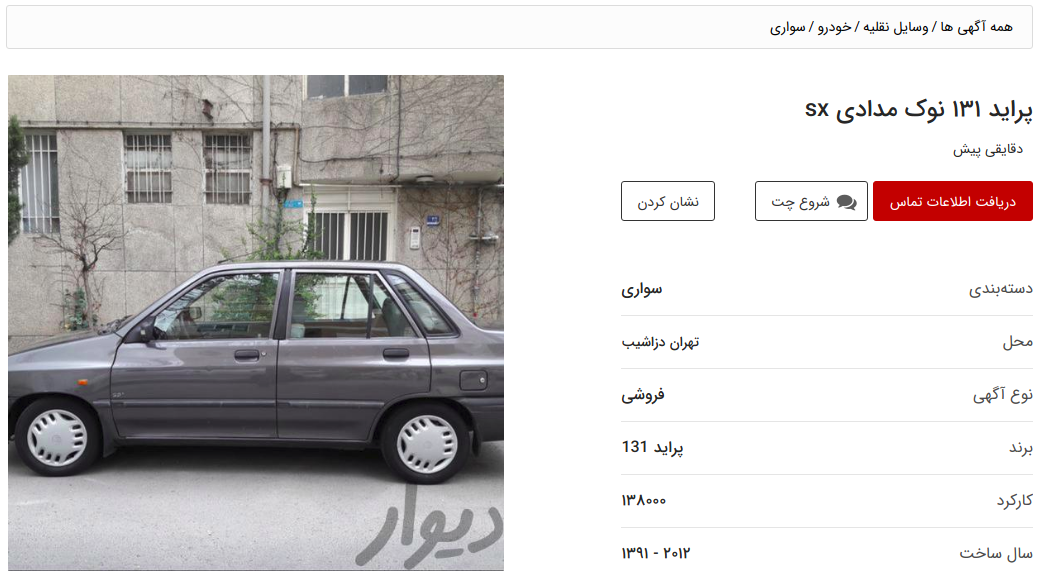
\includegraphics[height=\linewidth]{images/post1.png}
				
\includegraphics[width=\linewidth]{images/post2.png}
				
\includegraphics[width=\linewidth]{images/post3.png}
			\end{column}
		\end{columns}		
	}
	\frame{
		\frametitle{Columns}
		\begin{AutoMultiColItemize}
			\item id
			\item archive\_by\_user
			\item published\_at
			\item  \textbf <2> {cat1}
			\item  \textbf <2> {cat2}
			\item  \textbf <2> {cat3}
			\item city
			\item  \textbf <2> {title}
			\item  \textbf <2> {desc}
			\item price
			\item image\_count
			\item platform
			\item mileage
			\item brand
			\item year
			\item type
		\end{AutoMultiColItemize}
	}
%	\frame{
%		\frametitle{Title, Description, and Category}
%		\begin{tabular}{l|l|l|l|l}
%			\textbf{Title} & \textbf{Description} & \textbf{Cat1} & \textbf{Cat2} & \textbf{Cat3}\\
%			\hline
%			1&2&3&4&5
%		\end{r}
%		\\Some text
%	}
	\section{The Problem: Categorization}
		\frame{
			\frametitle{The Problem: Categorization}
			\begin{itemize}
				\item <2-> We need to categorize posts based on other posts features;
				\item <3-> We only use text features(title \& description)!
			\end{itemize}
		}
		%\subsection{Features}
			\frame{
				\frametitle{Features}
				\begin{center}
					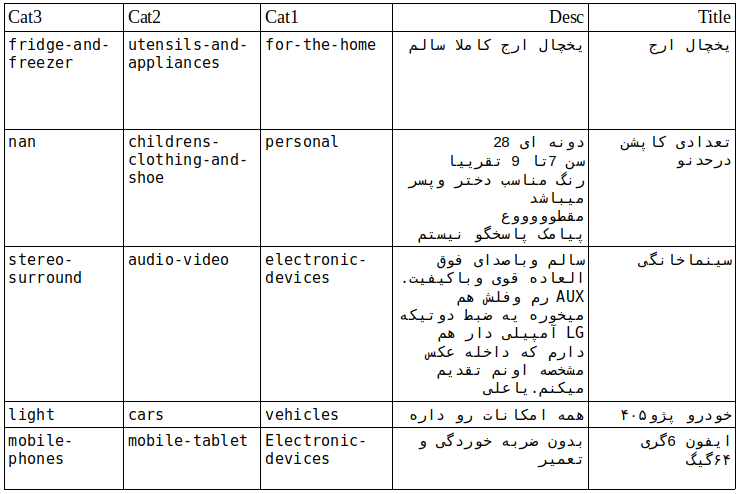
\includegraphics[width=.8\linewidth]{images/post_table.png}
				\end{center}
			}
		%\subsection{No. of Classes}
			\frame{
				\frametitle{No. of Classes}
				\begin{itemize}
					\item We concatenate three category columns into one; for example:
					{\begin{tabular}{lll|l}
						cat1&cat2&cat3&concatenate\\ \hline
						vehicles&cars&light&vehicles::cars::light
					\end{tabular}}
					\item Then, we have 87 unique combinations of categories, eg. 87 classes in our classification task.
				\end{itemize}
			}
	\section{Feature Extraction}
	\frame{
		\frametitle{Feature Extraction}
		Feature extraction is a dimensionality reduction process, where an initial set of raw variables is reduced to more manageable groups (features) for processing, while still accurately and completely describing the original data set.
	}
		\subsection{Tf-idf Vectorizer}
		\frame{
			\frametitle{Tf-idf Vectoizer}
			\begin{itemize}
				\item Tf-idf stands for term frequency-inverse document frequency
				\item a statistical measure used to evaluate how important a word is to a document in a collection or corpus
				\item the tf-idf weight is composed by two terms:
					\scriptsize\begin{description}
						\item [TF] \textbf{Term Frequency}, which measures how frequently a term occurs in a document.
						\begin{equation*}
						TF(t) = \frac{Number\ of\ times\ term\ t\ appears\ in\ a\ document}{Total\ number\ of\ terms\ in\ the\ document}
						\end{equation*}
						\item [IDF] \textbf{Inverse Document Frequency}, which measures how important a term is
						\begin{equation*}
						IDF(t) = \ln{\frac{Total\ number\ of\ documents}{Number\ of\ documents\ with\ term\ t\ in\ it}}
						\end{equation*}
					\end{description}
			\end{itemize}
		}
		\frame{
			\frametitle{Tf-idf Vectorizer: An Example}
			Consider a document containing 100 words wherein the word \textit{cat} appears 3 times. The term frequency (i.e., tf) for cat is then $tf(cat) = \frac{3}{100} = 0.03$. Now, assume we have 10 million documents and the word cat appears in one thousand of these. Then, the inverse document frequency (i.e., idf) is calculated as $idf(cat) = \ln{\frac{10,000,000}{1,000} = 4}$. Thus, the Tf-idf weight is the product of these quantities: $tf\--idf(cat) = 0.03 * 4 = 0.12$.
		}
		\subsection{Count Vectorizer}
		\frame{
			\frametitle{Vectorizing the Text: Count Vectorizer}
			An example: We want to vectorize these 4 sentences\footnote{Example from \href{https://github.com/rahulvasaikar/Bag-of-words}{Rahul Vasaikar}}:\\
			\begin{enumerate}
				\item Hello, how are you!
				\item Win money, win from home.
				\item Call me now
				\item Hello, Call you tomorrow?
			\end{enumerate}
		}
		\frame{
			\frametitle{Vectorizing the Text: Count Vectorizer}
			\begin{enumerate}
				\item We first build a vocabulary:\\
				\begin{math}
				vocabulary = \left\{are, call, from, hello, home, how, me, money, now, tomorrow, win, you\right\}
				\end{math}
				\item Then, we vectorize each sentence based on the occurness of each word:
				\scriptsize\begin{tabular}{l|llllllllllll}
					& are & call & from & hello & home & how & me & money & now & tom... & win & you \\\hline
					1       & 1   & 0    & 0    & 1     & 0    & 1   & 0  & 0     & 0   & 0        & 0   & 1   \\
					2 & 0   & 0    & 1    & 0     & 1    & 0   & 0  & 1     & 0   & 0        & 2   & 0   \\
					3               & 0   & 1    & 0    & 0     & 0    & 0   & 1  & 0     & 1   & 0        & 0   & 0   \\
					4 & 0   & 1    & 0    & 1     & 0    & 0   & 0  & 0     & 0   & 1        & 0   & 1  
				\end{tabular}
			\end{enumerate}
		}
		\subsection{Embedding}
		\frame{
			\frametitle{Word Embedding}
			\begin{quote}
				… when the input to a neural network contains symbolic categorical features (e.g. features that take one of k distinct symbols, such as words from a closed vocabulary), it is common to associate each possible feature value (i.e., each word in the vocabulary) with a d-dimensional vector for some d. These vectors are then considered parameters of the model, and are trained jointly with the other parameters.
			\end{quote}
		— Page 49, \href{http://amzn.to/2wycQKA}{Neural Network Methods in Natural Language Processing}, 2017.
		}
		\frame{
			\frametitle{Word Embedding}
			It requires that document text be cleaned and prepared such that each word is one-hot encoded. The size of the vector space is specified as part of the model, such as 50, 100, or 300 dimensions. The vectors are initialized with small random numbers. \textbf{The embedding layer is used on the front end of a neural network and is fit in a supervised way using the Backpropagation algorithm}.\footnote{From the article \href{https://machinelearningmastery.com/what-are-word-embeddings/}{What Are Word Embeddings for Text?
			}}
		}
		\frame{
			\frametitle{One-Hot Encoding for Word Embedding}
			\begin{enumerate}
				\item Hello, how are you!
				\item Win money, win from home.
				\item Call me now
				\item Hello, Call you tomorrow?
			\end{enumerate}
			{\small\begin{math}
			vocabulary = \left\{are, call, from, hello, home, how, me, money, now, tomorrow, win, you\right\}
			\end{math}}\\
		{\tabcolsep=0.11cm\begin{tabular}{l|cccccccccccc}
			Word & are & call & from & hello & home & how & me & money & now & tomorrow & win & you\\
			\hline
			Value & 1 & 2 & 3 & 4 & 5 & 6 & 7 & 8 & 9 & 10 & 11 & 12
		\end{tabular}}
		{\begin{tabular}{l|lllll}
			Sentence \\ \hline
			Hello, how are you! & 4&6&1&12&0\\
			Win money, win from home. & 11&8&11&3&5\\
			Call me now & 2&7&9&0&0\\
			Hello, Call you tomorrow? & 4&2&12&10&0
		\end{tabular}}
		}
		\frame{
			\frametitle{Number of Parameters}
			Let's say that we want to embed sentences(or words) into a $\mathbb{R}^n$ vector space. If m is the size of vocabulary, our Embedding layer has $m*n$ parameters that can be fitted in a supervised way using the Backpropagation.
		}
		
	\section{Classification Algorithms}
	\frame{
		\frametitle{Classification Algorithms}
		We used different classifiers and applied different models on the data. The classifiers we tested are:
			\begin{itemize}
				\item Naive Bayes
				\item Linear Support Vector Machine(SVM)
				\item Passive Aggressive Classifier
				\item Convolutional Neural Network(CNN)
			\end{itemize}
	}
		\subsection{Naive Bayes}
		\frame{
			\frametitle{Naive Bayes Classifier}
			\begin{columns}
				\begin{column}{.5\textwidth}
					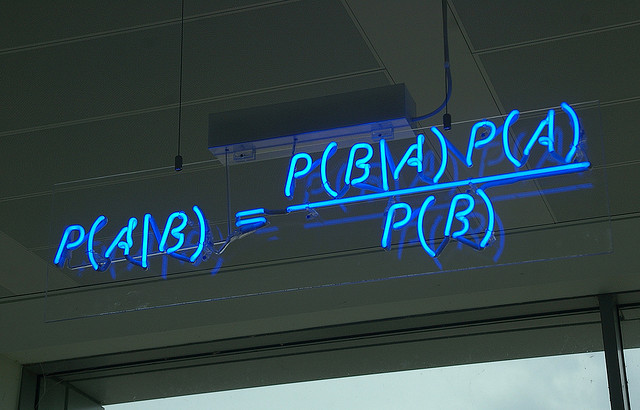
\includegraphics[width=\linewidth]{images/bayes_formula.jpg}
					\begin{center}
						Photo by \href{https://www.flickr.com/photos/mattbuck007/3676624894}{Matt Buck}
					\end{center}
				\end{column}
				\begin{column}{.5\textwidth}
					\begin{center}
						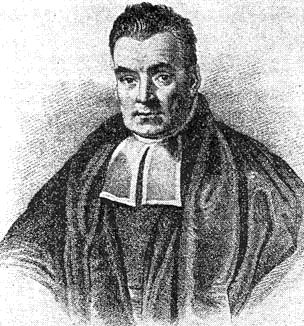
\includegraphics[width=.8\linewidth]{images/Thomas_Bayes.png}
					\end{center}
				\end{column}
			\end{columns}
		}
			\frame{
				\frametitle{Bayes Classifier: Naive One!}
				It is possible to show that accuracy is minimized, on average, by a
				very simple classifier that assigns each observation to the most likely class,
				given its predictor values. In other words, we should simply assign a test
				observation with predictor vector $x_0$ to the class j for which\\
				\begin{center}
					\begin{math}
						P\left(Y=j\ \middle|\ \mathbf{X}=\mathbf{x}\right)
					\end{math}
				\end{center}
				is largest.
			}
			\frame{
				\frametitle{Bayes Classifier: Naive One!}
				We make two assumptions:
				\begin{enumerate}
					\item $X_1, X_2, \ldots, and\ X_m$ are independent from each other;
					\item $X_1, X_2, \ldots, X_m\mid Y \thicksim MN(\cdot, p_1, p_2, \ldots, p_m)$
				\end{enumerate}
				{\scriptsize\begin{align*}
					P(Y=j\mid\mathbf{X}=(x_1, x_2, \ldots, x_m))
					 &= \frac{P(\mathbf{X}=(x_1, x_2, \ldots, x_m)\mid Y=j)\cdot P(Y=j)}{P(\mathbf{X}=\mathbf{x})}\\
					 &= \frac{P(X_1=x_1\mid Y=j)\cdot\ldots\cdot P(X_m=x_m\mid Y=j)\cdot P(Y=j)}{P(\mathbf{X}=\mathbf{x})}.
				\end{align*}}
				\scriptsize\begin{align*}
					\hat{y} = \argmax_{j\in classes} \frac{P(X_1=x_1\mid Y=j)\cdot\ldots\cdot P(X_m=x_m\mid Y=j)\cdot P(Y=j)}{P(\mathbf{X}=\mathbf{x})}\\
					=\argmax_{j\in classes} P(X_1=x_1\mid Y=j)\cdot\ldots\cdot P(X_m=x_m\mid Y=j)\cdot P(Y=j).
				\end{align*}
			}
			\frame{
				\frametitle{Hyperparameters}
				Two important hyperparameters:
				\begin{enumerate}
					\item Size of the vocabulary;
					\item Laplace/ Lidstone smoothing parameter($\alpha$).
					\item Prior
				\end{enumerate}
			}
			\frame{
				\frametitle{Size of Vocabulary}
				We can determine the size of our vocabulary.
				\begin{center}
					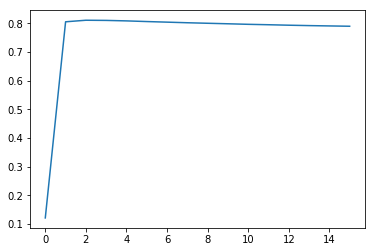
\includegraphics[width=.6\linewidth]{images/plot1.png}\\
				\end{center}
				It is convex!
			}
			\frame{
				\frametitle{Laplace/ Lidstone Smoothing Parameter($\alpha$)}
				\begin{center}
					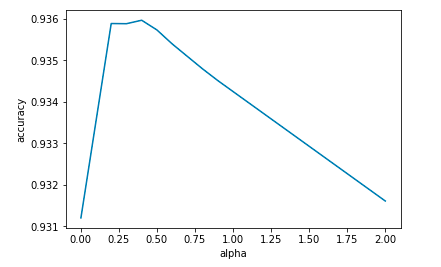
\includegraphics[width=.6\linewidth]{images/plot2.png}\\
					It is convex!
				\end{center}
			}
			\frame{
				\frametitle{Whether Use Prior or Not}
				\begin{center}
					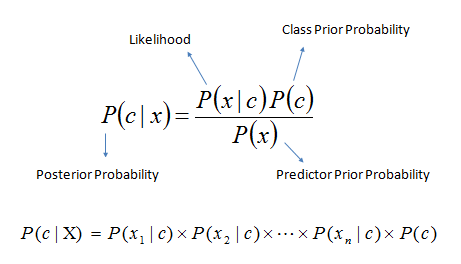
\includegraphics[width=\linewidth]{images/prior.png}
				\end{center}
			}
			\frame{
				\frametitle{Whether Use Prior or Not}
				According to the \href{https://research.cafebazaar.ir/visage/divar_datasets/}{dataset webpage}, \textbf{distribution of dataset posts in different groups does not resemble the actual distributions}. So, if we fit a prior our accuracy with cross-validation increases, but it doesn't mean that our model is good; because model fits a wrong prior.\\ So we should not fit a prior(e.g. use an uninformative one).
			}
			\frame{
				\frametitle{Bayes Classifier: Naive One!}
				Let's dive into code!
			}
		\subsection{CNN}
		
			\frame{
				\frametitle{CNN Over Embedding Layer}
				\begin{center}
					
\includegraphics[height=8cm]{images/nn.png}
				\end{center}
			}
			\frame{
				\frametitle{CNN Over Embedding Layer}
				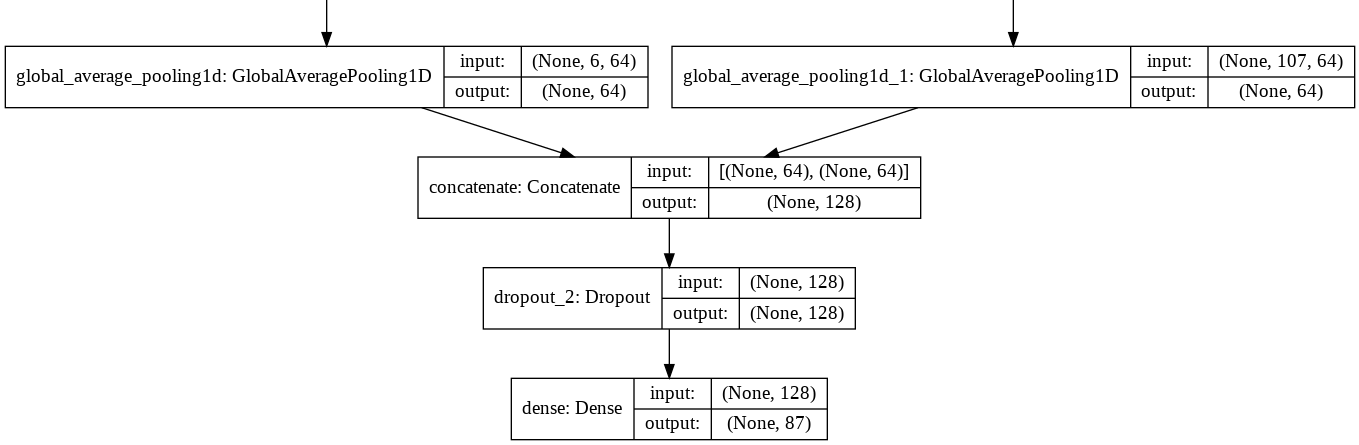
\includegraphics[width=\linewidth]{images/concat.png}
			}
			\frame{
				\frametitle{CNN Over Embedding Layer}
				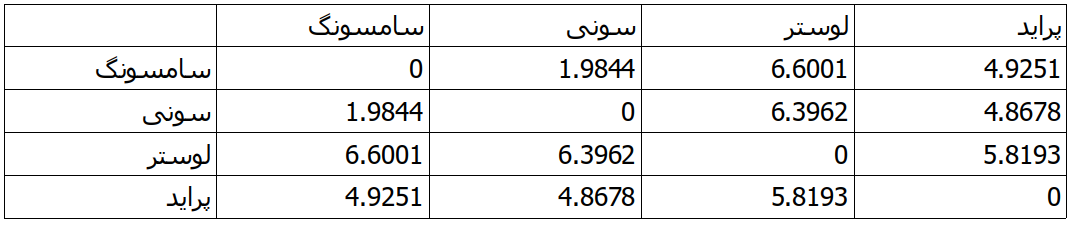
\includegraphics[width=\linewidth]{images/comp_table.png}
			}
		\subsection{Linear SVM}
		\frame{
			\frametitle{Support Vector Machines}
			\begin{columns}
				\begin{column}{.5\textwidth}
					SVM constructs a hyperplane in multidimensional space to separate different classes. SVM generates optimal hyperplane in an iterative manner, which is used to minimize an error. The core idea of SVM is to find a maximum marginal hyperplane(MMH) that best divides the dataset into classes.
				\end{column}
				\begin{column}{.5\textwidth}
					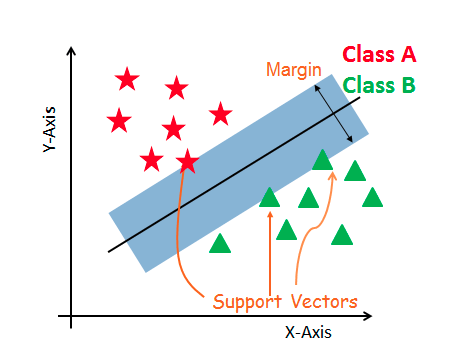
\includegraphics[width=\linewidth]{images/svm1.png}
				\end{column}
			\end{columns}
		}
		\frame{
			\frametitle{How does SVM work?}
			The main objective is to segregate the given dataset in the best possible way. The distance between the either nearest points is known as the margin. The objective is to select a hyperplane with the maximum possible margin between support vectors in the given dataset. SVM searches for the maximum marginal hyperplane in the following steps:
		}
		\frame{
			\frametitle{How does SVM work?}
			\begin{enumerate}
			\begin{columns}
				\begin{column}{.45\textwidth}
					\item Generate hyperplanes which segregates the classes in the best way. Left-hand side figure showing three hyperplanes black, blue and orange. Here, the blue and orange have higher classification error, but the black is separating the two classes correctly.
					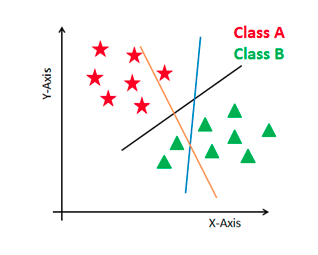
\includegraphics[width=.9\linewidth]{images/svm2.png}
				\end{column}
				\begin{column}{.45\textwidth}
					\item Select the right hyperplane with the maximum segregation from the either nearest data points as shown in the right-hand side figure.\\[1.1cm]
					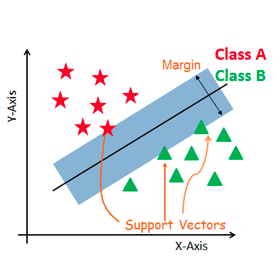
\includegraphics[width=.9\linewidth]{images/svm3.png}
				\end{column}
			\end{columns}
			\end{enumerate}
		}
		\frame{
			\frametitle{Linear SVM}
			Let's dive into code!
		}
		\subsection{Passive Aggressive Classifier}
		\frame{
			\frametitle{Passive Aggressive}
			\begin{itemize}
				\item A margin based online learning algorithm
				\item Perfect for classifying massive streams
				\item Easy to implement and very fast
				\item \textbf{Passive}: if correct classification, keep the model;
				\item \textbf{Aggressive}: if incorrect classification, update to adjust to this misclassified example
				\item See \url{http://koaning.io/passive-agressive-algorithms.html} for further reading
				\item Link to the original paper: \url{http://jmlr.csail.mit.edu/papers/volume7/crammer06a/crammer06a.pdf}
			\end{itemize}
		}
		\frame{
			\frametitle{Passive Aggressive}
			Let's dive into code!
		}
	\section{A Comparison among Models}
	\subsection{Ensemble Learning}
	\frame{
		\frametitle{Ensemble Learning}
		\begin{columns}
			\begin{column}{.5\textwidth}
				\begin{itemize}
					\item CountVectorizer + MutinomialNB
					\item TfidfVectorizer + MutinomialNB
					\item CountVectorizer + ComplementNB
					\item TfidfVectorizer + ComplementNB
					\item CountVectorizer + SVM(Hinge)
					\item CountVectorizer + SVM(HingeSq.)
					\item TfidfVectorizer + SVM(Hinge)
					\item TfidfVectorizer + SVM(HingeSq.)
				\end{itemize}
			\end{column}
			\begin{column}{.25\textwidth}
				PCA(100PC) + Structured data
			\end{column}
			\begin{column}{.25\textwidth}
				5-Layer Perceptron
			\end{column}
		\end{columns}
	}
	\subsection{Comparison}
	\frame{
		\frametitle{Models Comparison}
		\begin{table}[]
			\begin{tabular}{|l||l|l|l|l|}
				\hline
				Name     & Accuracy & Vectorizer     & Classifier        & Text Strategy    \\ \hline
				SVM      & 93.78    & Tf-Idf         & SVM               & Dual Vectorizers \\ 
				Ensemble & 93.19    & Count + Tf-Idf & Various!          & Concat Text      \\ 
				P-A      & 92.80    & Count          & Passive-Agressive & Concat Text      \\ 
				CNN\footnote{Trained with 80\% of data!}      & 90.50     & Embedding      & CNN               & Dual CNN         \\ \hline
			\end{tabular}
		\end{table}
	}
	
	\section{The End}
	\frame{
		\frametitle{Thanks for your attention!}
		\begin{itemize}
			\item Codes and slides(in MLSP GitHub):\\
			\url{https://github.com/ut-mlsp/Text-classification-crash-course}
			\item Divar posts dataset:\\
			\url{https://research.cafebazaar.ir/visage/divar_datasets/}
			\item Any questions?
		\end{itemize}
		
	}
\end{document}
